% Op icon: build surface from selected lines — a closed loop of marked segments, lightly shaded.
\documentclass[tikz,border=2mm]{standalone}
\usetikzlibrary{arrows.meta,calc,shapes.geometric}
\begin{document}
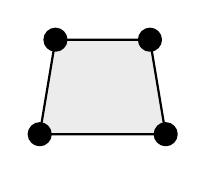
\begin{tikzpicture}[line width=1.3pt, line cap=round, line join=round, >=Stealth, x=1mm,y=1mm]
  \draw[thick, fill=gray!15] (-8,-6) -- (8,-6) -- (6,6) -- (-6,6) -- cycle;
  \foreach \p in {(-8,-6),(8,-6),(6,6),(-6,6)} { \filldraw \p circle (1.3); }
\end{tikzpicture}
\end{document}
